% !TeX root = ../tesis.tex

\chapter{Esparcimiento de luz por partículas}
\label{chapter:theory}

\vspace*{7em}

En este capítulo


\section{Fundamentos}
\label{section:basics}
Todos los fenómenos electromagnéticos tienen su origen en una única interacción fundamental: la fuerza de Lorentz. Esta fuerza describe cómo actúa un campo electromagnético sobre una partícula cargada en movimiento. Si una partícula de carga \( q \) se desplaza con velocidad \( \vb{v} \) en presencia de un campo eléctrico \( \vb{E} \) y un campo magnético \( \vb{B} \), la fuerza que experimenta está dada por:
%
\begin{equation}
	\vb{F}=q(\vb{E}+\vb{v}\times\vb{B}).
	\label{eq:lorentzforce} 
\end{equation}
%
La fuerza de Lorentz junto con las ecuaciones de Maxwell, describen a la electrodinámica clásica, que se centra en el origen y el comportamiento de los campos $\vb{E}$ y $\vb{B}$ \cite{griffithsIntroductionElectrodynamics2023}. En unidades del Sistema Internacional, dichas ecuaciones se expresan en forma diferencial como:
\cite{griffithsIntroductionElectrodynamics2023}
%
	\begin{subequations} \label{eqs:Maxwell}
	\begin{tcolorbox}[
	ams align, breakable]
	\nabla \cdot\vb{E} &= \frac{\rho_{tot}}{\varepsilon_0}, &\mbox{(Ley de Gauss eléctrica)}  
	\label{seq:GE} \\
	\nabla \cdot\vb{B} &= 0,						&\mbox{(Ley de Gauss magnética)}   
	\label{seq:GM} \\
	\nabla \times\vb{E} &= -\pdv{\vb{B}}{t}, 	&\mbox{(Ley de Faraday-Lenz)}		
	\label{seq:FL}\\
	\nabla \times\vb{B} &= \mu_0 \vb{J}_{tot} +\varepsilon_0\mu_0 \pdv{\vb{E}}{t}, &
	\mbox{(Ley de Ampère-Maxwell)} \label{seq:AM}
	\end{tcolorbox}\end{subequations}\noindent
%
donde $\rho_{tot}$ representa a la densidad de carga volumétrica y $\vb{J}_{tot}$ a la densidad de corriente volumétrica; $\epsilon_0$ a la permitividad eléctrica en el vacío y $\mu_0$ a la permeabilidad magnética en el vacío. 

En ausencia de fuentes externas (\( \rho_{\text{tot}} = 0 \), \( \vb{J}_{\text{tot}} = 0 \)), los campos electromagnéticos pueden desacoplarse y satisfacer la ecuación de onda de Helmholtz al aplicar la transformada de Fourier temporal ~\cite{jacksonClassicalElectrodynamics2021}. Una de las soluciones de esta ecuación son las ondas planas, que representan la propagación de una onda monocromática en una dirección definida

	\begin{subequations}%
	\eqhalf{\vb{E}(\vb{r},t) =\vb{E_0}e^{i(\vb{k}\cdot\vb{r} -\omega t)},}\label{seq:E_plana}% 
	\eqhalf{\vb{B}(\vb{r}, t) =\vb{B_0}e^{i(\vb{k}\cdot\vb{r} -\omega t)},}	\label{seq:B_plana}
	\label{eqs:ondasPlanas}\end{subequations}\vspace*{-1em}
		
\noindent donde $\vb{E}_0$ y $\vb{B}_0$ corresponden a las amplitudes de los campos, $\omega$ la frecuencia angular de la onda y $\vb{k}$ el vector de onda. Para que se satisfagan las Ecs. \eqref{eqs:ondasPlanas}, se tiene que cumplir la relación de dispersión dada por el número de onda $k=\sqrt{\mu\varepsilon}\;\omega$, donde $\varepsilon$ y $\mu$ corresponden a la permitividad eléctrica y la permeabilidad magnética del medio y son en general, funciones complejas dependientes de $\omega$. \cite{jacksonClassicalElectrodynamics2021}. La relación de dispersión se puede reescribir en términos del índice de refracción del material dado por
%
\begin{tcolorbox}[ams align]
	n(\omega) = \sqrt{\dfrac{\varepsilon\mu(\omega)}{\varepsilon_0\mu_0 }},
	\label{eq:indice} 
\end{tcolorbox}
%	
\noindent con lo que se obtiene,
%
\begin{equation}
	k(\omega) =\dfrac{\omega n(\omega)}{c},
	\label{eq:numero_onda} 
\end{equation}

\noindent donde $c=1/\sqrt{\epsilon_0\mu_0}$ es la velocidad de la luz en el vacío.

Al analizar la energía total almacenada en los campos electromagnéticos y el trabajo que estos realizan sobre una distribución de cargas y corrientes, se establece el teorema del trabajo y la energía. A partir de este teorema, se introduce el concepto de energía transportada por los campos por unidad de tiempo y por unidad de área, el cual está representado por el vector de Poynting, $\vb{S}$, dado por \cite{griffithsIntroductionElectrodynamics2023}

\begin{tcolorbox}[ams align]
	\vb{S}=\frac{1}{\mu_0}(\vb{E}\times\vb{B}),
	\label{eq:vect_Poynting} 
\end{tcolorbox}


Las Ecs. \eqref{eqs:Maxwell} determinan los campos que surgen a partir de corrientes y cargas presentes en la materia. No obstante, dichas ecuaciones no explican el origen de estas corrientes y cargas. Por ello, es necesario complementarlas con ecuaciones llamadas \textit{relaciones constitutivas}, que describen cómo responde la materia ante la acción de los campos. Para un medio lineal, homogéneo e isótropo, las relaciones constitutivas están dadas por \cite{novotnyPrinciplesNanooptics2012}
%
\begin{subequations} \label{eqs:Constitutivas}
	\begin{tcolorbox}[
		ams align, breakable]
		\vb{D}(\vb{r},\omega) &= \epsilon(\omega)\; \vb{E}(\vb{r},\omega), \\
		\label{seq:D} 
		\vb{B}(\vb{r},\omega) &= \mu(\omega) \vb{H}(\vb{r},\omega),\\
		\label{seq:B} 
		\vb{J}(\vb{r},\omega) &= \sigma (\omega) \vb{E}(\vb{r},\omega),
		\label{seq:J}\end{tcolorbox}\end{subequations}\noindent
%	
donde $\vb{D}$ corresponde al vector de desplazamiento eléctrico, $\vb{H}$ al campo H, $\vb{J}$ a la densidad volumétrica de corriente  y $\sigma$ corresponde a la conductividad eléctrica.

Dadas las relaciones anteriores, la parte temporal puede ser construida empleando la transformada de Fourier\footnote{Sea $F(t)$ una función real dependiente del tiempo, la transformada de Fourier $\mathcal{F}(\omega)$ de $F(t)$ se define como $1/\sqrt{2\pi}\int_{-\infty}^{\infty}F(t)e^{i\omega t} \text{d}t$. Mientras que la transformada de Fourier inversa $\mathcal{F}^{-1}$ es $1/\sqrt{2\pi}\int_{-\infty}^{\infty}\mathcal{F}(\omega)e^{-i\omega t} \text{d}\omega$ }. La transformada de Fourier para $\vb{D}$ está dada por
%
\begin{equation}
	\vb{D}(\vb{r},t)=\frac{1}{\sqrt{2\pi}}\int_{-\infty}^{\infty}\vb{D}(\vb{r},\omega)e^{-i\omega t}\text{d}\omega,\label{eq:TF}
\end{equation}
%
mientras que la transformada de Fourier inversa está dada por
%
\begin{equation}
	\vb{D}(\vb{r},\omega)=\frac{1}{\sqrt{2\pi}}\int_{-\infty}^{\infty}\vb{D}(\vb{r},t')e^{i\omega t'}\text{d}t'.\label{eq:TFI}
\end{equation}
%
Al sustituir la Ec. \eqref{seq:D} en la Ec. \eqref{eq:TF}, se obtiene
%
\begin{equation}
	\vb{D}(\vb{r},t)=\frac{1}{\sqrt{2\pi}}\int_{-\infty}^{\infty}\varepsilon(\omega)\vb{E}(\vb{r},\omega)e^{-i\omega t}\text{d}\omega,\label{eq:TF_D_intermedia_1}
\end{equation}
%
y al sustituir la transformada de Fourier de $\vb{E}(\vb{r},t)$, se obtiene:
%
\begin{equation}
	\vb{D}(\vb{r},t)=\frac{1}{\sqrt{2\pi}}\int_{-\infty}^{\infty}\varepsilon(\omega)e^{-i\omega t}\text{d}\omega\int_{-\infty}^{\infty}e^{i\omega t'}\vb{E}(\vb{r},t')\text{d}t'.\label{eq:TF_D_intermedia_2}
\end{equation}
%
Considerando que los órdenes de integración se pueden intercambiar y realizando el cambio de variable $\tau=t-t'$, la Ec. \eqref{eq:TF_D_intermedia_2} se reescribe como
%
\begin{equation}
	\vb{D}(\vb{r},t)=\frac{1}{\sqrt{2\pi}}\int_{-\infty}^{\infty}\int_{-\infty}^{\infty}\varepsilon(\omega)\vb{E}(\vb{r},t') e^{i\omega \tau} \text{d}\omega \text{d}t'.\label{eq:TF_D_intermedia_2}
\end{equation}
%
Al emplear la función constante
\begin{equation}
	\mathcal{F}[1]=\int_{-\infty}^{\infty}e^{-i\omega\tau}=\delta(\tau),
\end{equation}
donde $\delta(\tau)$ es la delta de Dirac, que cumple con
\begin{equation}
	\int_{-\infty}^{\infty}f(\tau)\delta(\tau)\text{d}\tau=f(0),
\end{equation}
entonces, se reescribe al campo eléctrico como
\begin{equation}
	\vb{E}(\vb{r},t)=\int_{-\infty}^{\infty}\vb{E}(\vb{r},t-\tau)\delta(\tau)=\frac{1}{2\pi}\int_{-\infty}^{\infty}\int_{-\infty}^{\infty}\vb{E}(\vb{r},t-\tau)\e^{-i\omega\tau}\text{d}\omega\text{d}\tau.
\end{equation}
%
Al sumar $\vb{E}(\vb{r},t')-\vb{E}(\vb{r},t')$ y multiplicar por $\varepsilon_0/\varepsilon_0$ a la Ec. \eqref{eq:TF_D_intermedia_2}, simplificando se obtiene
%
\begin{equation}
	\vb{D}(\vb{r},t)=\varepsilon_0\left[\vb{E}(\vb{r},t)+\int_{-\infty}^{\infty}G(\tau)\vb{E}(\vb{r},t-\tau)\text{d}\tau\right],\label{eq:TF_D_final}
\end{equation}
%
donde $G(\tau)$ es la transformada de Fourier de la susceptibilidad eléctrica $\chi_e=\varepsilon(\omega)/\varepsilon_0-1$
%
\begin{equation}
	G(\tau)=\frac{1}{2\pi}\int_{-\infty}^{\infty}\left[\frac{\varepsilon(\omega)}{\varepsilon_0}-1\right]e^{-i\omega\tau}\tex{d}\omega
	\label{eq:G_tdependent}
\end{equation}
%
Las Ecs. \eqref{eq:TF_D_final} y \eqref{eq:G_tdependent} muestran que el campo de desplazamiento eléctrico al tiempo $t$ depende del campo eléctrico en todos los demás tiempos $t'$. A esta característica, se le conoce como la no localidad temporal entre $\vb{D}$ y $\vb{E}$. Si $\varepsilon(\omega)$ es independiente del \omega, $G(\tau)=\delta(\tau)$, por lo que se obtiene una respuesta instantánea, mientras que si sí depende de $\omega$, $G(\tau)$ es distinta de cero para todos los valores de $\tau$ distintos de cero.





A partir de la forma integral de las ecuaciones de Maxwell, se deducen las condiciones de frontera sobre los campos electromagnéticos al atravesar una interfaz entre dos medios distintos. Cada uno de los medios está caracterizado por una función dieléctrica y una permeabilidad magnética ($\epsilon_1, \mu_1$ para el medio 1 y $\epsilon_2, \mu_2$ para el medio 2). Para deducirlas, se considera un prisma de altura $\delta$ y área transversal $A$ [Fig. \ref{cond_perp}], y un circuito rectangular de altura $\delta$ y longitud $l$ [Fig. \ref{cond_par} ]. Bajo las suposiciones de medios lineales, homogéneos e isótropos, y en ausencia de fuentes externas ($\sigma_{\text{ext}} = 0$, $\vb{K}_{\text{ext}} = 0$), al emplear de las ecuaciones de Maxwell en su forma integral y las Ecs. \eqref{eqs:Constitutivas}, se obtienen a las siguientes condiciones de frontera:

%
\begin{subequations} \label{cond_frontera}
	\begin{tcolorbox}[
		ams align, breakable]
		\eqhalf{\epsilon_1E_1^{\perp}-\epsilon_2E_2^{\perp}= 0,}%
		\eqhalf{\vb{E}_1^{\parallel}-\vb{E}_1^{\parallel}=0,}\\
		\eqhalf{B_1^{\perp}-B_2^{\perp}=0,}%
		\eqhalf{\frac{\vb{B}_1}{\mu_1}-\frac{\vb{B}_2}{\mu_2}=0,}		\label{seq:D} \end{tcolorbox}\end{subequations}\noindent

%
\begin{figure}[H]
	\centering
	\sidesubfloat[First image]{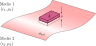
\includegraphics[width=0.4\textwidth]{../Figuras/condiciones_contorno_perp}\label{cond_perp}}
	\sidesubfloat[Second image]{\includegraphics[width=0.4\textwidth]{../Figuras/condiciones_contorno_par}\label{cond_par}}
	\caption{Esquema de una interfaz que separa dos medios distintos. El medio 1 se encuentra caracterizado por una función dieléctrica $\epsilon_1$ y una permeabilidad magnética $\mu_1$, mientras que el medio 2 se encuentra caracterizado por una función dieléctrica $\epsilon_2$ y una permeabilidad magnética $\mu_2$. \textbf{a)} Interfaz con una densidad superficial de carga $\sigma_{tot}$ que es atravesada por un prisma rectangular de altura $\delta$ y área $A$. \textbf{b)} Interfaz con una densidad de superficial de corriente $\vb{K}_{tot}$. La densidad de corriente atraviesa una superficie rectangular de altura $\delta$ y longitud $l$.}
	\label{condiciones_frontera}
\end{figure}
%
